\documentclass{article}


\usepackage{arxiv}

\usepackage[utf8]{inputenc} % allow utf-8 input
\usepackage[T1]{fontenc}    % use 8-bit T1 fonts
\usepackage{hyperref}       % hyperlinks
\usepackage{url}            % simple URL typesetting
\usepackage{booktabs}       % professional-quality tables
\usepackage{amsfonts}       % blackboard math symbols
\usepackage{nicefrac}       % compact symbols for 1/2, etc.
\usepackage{microtype}      % microtypography
\usepackage{lipsum}

\usepackage{amssymb}
\usepackage{lineno,hyperref}
\usepackage{amsmath}
\usepackage[makeroom]{cancel}
\usepackage{mathtools}
\usepackage{subeqnarray}
\usepackage[utf8]{inputenc}
\usepackage[english]{babel}
 
\usepackage[square,numbers]{natbib}
\bibliographystyle{abbrvnat}
 

\usepackage{graphics}
\usepackage[pdftex]{graphicx}
\usepackage{epsfig}

\usepackage{array}
\usepackage{wrapfig}
\usepackage{color}
\usepackage{lineno}
\usepackage{ragged2e}
\usepackage{subfig}
\usepackage{bm}
\usepackage{stmaryrd}

\usepackage{multirow}

\usepackage{soul}
%\usepackage{SIunits}
%\usepackage{psfig}
%\usepackage{boldfonts}
\usepackage{symbols}
\newtheorem{remark}{Remark}

\usepackage[export]{adjustbox}

\newtheorem{thm}{Theorem}
\newtheorem{lem}{Lemma}


\usepackage{xcolor,cancel}

\newcommand\hcancel[2][black]{\setbox0=\hbox{$#2$}%
\rlap{\raisebox{.45\ht0}{\textcolor{#1}{\rule{\wd0}{1pt}}}}#2} 

%\usepackage{boldfonts}
%\usepackage{symbols}

\usepackage{tikz, xcolor}
\usetikzlibrary{shapes.geometric}
\usetikzlibrary{shapes,arrows}
\usepackage{siunitx} 

\usepackage{geometry}
\geometry{
 a4paper,
 total={170mm,257mm},
left=20mm,
top=30mm,
right=20mm,
bottom = 40mm
}

\newcommand{\shlee}[1]{{\textcolor{blue}{#1}}}
\newcommand{\meen}[1]{{\textcolor{green}{#1}}}

\newcommand{\bdf}[2]{{\textup{\textsf{BDF}}_{#2}\left({#1}\right)}}
\newcommand{\BDF}[1]{\bdf{\left( #1 \right)}{2}}

\newcommand{\vertiii}[1]{{\left\vert\kern-0.25ex\left\vert\kern-0.25ex\left\vert #1 
    \right\vert\kern-0.25ex\right\vert\kern-0.25ex\right\vert}}
\def\p{\partial}
\newtheorem{form}{Formulation}

\usepackage{sectsty} 
\sectionfont{\large}

\title{Choice of interior penalty coefficient for interior penalty discontinuous Galerkin method by employing machine learning}


\author{
  Sanghynu Lee\thanks{Use footnote for providing further
    information about author (webpage, alternative
    address)---\emph{not} for acknowledging funding agencies.} \\
  Department of Computer Science\\
  Cranberry-Lemon University\\
  Pittsburgh, PA 15213 \\
  \texttt{hippo@cs.cranberry-lemon.edu} \\
  %% examples of more authors
   \And
 Elias D.~Striatum \\
  Department of Electrical Engineering\\
  Mount-Sheikh University\\
  Santa Narimana, Levand \\
  \texttt{stariate@ee.mount-sheikh.edu} \\
  \And
 John Doe \\
  Department of Electrical Engineering\\
  Mount-Sheikh University\\
  Santa Narimana, Levand \\
  \texttt{John@ee.mount-sheikh.edu} \\
  %% \AND
  %% Coauthor \\
  %% Affiliation \\
  %% Address \\
  %% \texttt{email} \\
  %% \And
  %% Coauthor \\
  %% Affiliation \\
  %% Address \\
  %% \texttt{email} \\
  %% \And
  %% Coauthor \\
  %% Affiliation \\
  %% Address \\
  %% \texttt{email} \\
}

\begin{document}
\maketitle

\begin{abstract}
\lipsum[1]
\end{abstract}


% keywords can be removed
\keywords{First keyword \and Second keyword \and More}


\section{Introduction}

Discontinuous Galerkin finite element method (DG) is employed for various realistic applications, especially with discontinuous coefficients. The main advantages for DG are XXX, YYY, and ZZZ. Mathematical analyses for stability and error convergence are shown in for elliptic problems in [citation]. 
These studies are proved under an assumption on the interior penalty, and it is   crucial to employ the interior penalty term being sufficiently large enough. 
Several studies of the lower bounds for the penalty parameter have been obtained in \cite{ainsworth2007posteriori,ainsworth2010fully,ainsworth2009constant,epshteyn2007estimation,shahbazi2005explicit}. Moreover, specific illustrations on the selection of the penalty parameters are shown in \cite{ainsworth2012note}.

%Recently, EG?

A lower bound for the standard DG was given for the case when there is an arbitrary number of hanging nodes in the mesh and elements of arbitrary nonuniform polynomial order in \cite{shahbazi2005explicit}.
This bound was improved upon in \cite{ainsworth2009constant} in the case when there was at most one hanging node per edge of each element, which lay at the midpoint of the edge. 
In cases where the diffusion coefficient is discontinuous, it has been suggested that a nonstandard DG is used in which a weighted interior penalty term is employed \cite{ern2008posteriori,ern2009discontinuous}. 
It is of considerable practical interest to
determine bounds on the interior penalty parameter sufficient for this variant of DG to give
a well-defined numerical approximation. 
A bound which is
applicable to the case when there is an arbitrary number of hanging nodes and elements may be of arbitrary nonuniform polynomial order is shown in  \cite{ainsworth2012note}.


Conclusion
\begin{itemize}
\item For Darcy with smooth coefficients : need a minimum $\beta$ but not the maximum for optimal convergence rate. However, the iterative solver is affected.
\item For Darcy with non-smooth coefficients : To observe sub-optimal convergence rate, minimum and maximum bound for $\beta$ is required. 
\item For Biot's equations : to avoid oscillations, optimal choice of $\beta$ is required. Here we employ SIPG and iterative solver. 
\end{itemize}

\section{Mathematical Model}
We consider the following elliptic system,  
\begin{equation}\label{eq-main}
\left\{ 
\begin{array}{rll} 
-\nabla \cdot \left( \bm{K} \nabla p \right)
&=  f
& \textrm{in}~\Omega, \\
u&=0& \textrm{on}~\partial \Omega,
\end{array}
\right.
\end{equation}
%%%%%%%%%%%%%%%%%%%%%%%%]
where a bounded, open, and convex domain is denoted by 
$\Omega \subset \mathbb{R}^d (d \in {2,3})$, $K\in \mathbb{R}^{d\times d}$ and $f \in L_2(\Omega)$.

Then the weak solution $p \in H_0^{1}(\Omega)$ 
of \eqref{eq-main} is given by 
\begin{equation}
\int_\Omega K \nabla p \nabla v \ dx = 
\int_\Omega f  v \ dx, \ \ \ \forall v \in H_0^1(\Omega)
\label{eq-weak}
\end{equation}
where $H_0^1(\Omega):= \{  v \in H^1(\Omega): v = 0 \text{ on } \partial \Omega \}$

\subsection{Biot's system for poroelasticity}

\section{Numerical Discretizations}
\subsection{Finite element approximations}
Let $\mathcal{T}_h$ be the shape-regular (in the sense of Ciarlet)  triangulation by a family of partitions of $\O$ into $d$-simplices $\K$ (triangles/squares in $d=2$ or tetrahedra/cubes in $d=3$). We denote by $h_{\K}$ the diameter of $\K$ and we set $h=\max_{\K \in \Th} h_{\K}$.  
Also we denote by $\Eh$ the set of all edges and by $\Eho$ and $\mathcal{E}^{\partial}_{h}$ the collection of all interior and boundary edges, respectively. 
In the following notation, we assume edges for two dimension but the results hold analogously for faces in three dimensional case.
The space $H^{s}(\Th)$ $(s\in \mathbb{R})$ is the set of element-wise $H^{s}$ functions on $\mathcal{T}_h$, and $L^{2}(\Eh)$ refers to the set of functions whose traces on the elements of $\Eh$ are square integrable. Let $\mathbb{Q}_l(\K)$ denote the space of polynomials of partial degree at most $l$. 
Throughout the paper, we use the standard notation for Sobolev spaces and their norms. For example, let $E \subseteq \Omega$, then $\|\cdot\|_{1,E}$ and $|\cdot|_{1,E}$ denote the $H^1(E)$ norm and seminorm, respectively. 
For simplicity, we eliminate the subscripts on the norms if $E = \Omega$.
For any $e \in \Eho$, let $\K^{+}$ and $\K^{-}$ be two neighboring elements such that  
$$
e = \partial \K^{+}\cap \partial \K^{-}
$$
and we denote by $h_{e}$ the length of the edge $e$. 
Let $\bm{\mathrm{n}}^{+}$ and $\bm{\mathrm{n}}^{-}$ be the outward normal unit vectors to  $\partial T^+$ and $\partial T^-$, respectively ($\bm{\mathrm{n}}^{\pm} :=\bm{\mathrm{n}}_{|\K^{\pm}}$). 
For any given function $\xi$ and vector function $\bm{\xi}$, defined on the triangulation $\mathcal{T}_h$, we denote $\xi^{\pm}$ and $\bm{\xi}^{\pm}$ by the restrictions of $\xi$ and $\bm{\xi}$ to $T^\pm$, respectively. 

Next, we define the  average $\av{\cdot}$ as follows: for $\zeta \in L^2(\mathcal{T}_h)$ and $\bm{\tau} \in L^2(\mathcal{T}_h)^d$,
\begin{equation}\label{av-w}
\av{\zeta} := \frac{1}{2} (\zeta^+ + \zeta^- )
\quad \mbox{ and } \quad 
\av{\bm{\tau}} := \frac{1}{2} (\bm{\tau}^+ +   \bm{\tau}^-) \quad \mbox{on } e\in
\Eho.
\end{equation}
On the other hand, for $e \in \mathcal{E}^{\partial}_{h}$, we set $\av{\zeta} :=   \zeta$ and $\av{\bm{\tau}} :=  \bm{\tau}$. 
The jump across the interior edge will be defined as 
\begin{align*}
\jump{\zeta} = \zeta^+\bm{\mathrm{n}}^++\zeta^-\bm{\mathrm{n}}^- \quad \mbox{ and } \quad \jtau = \bm{\tau}^+\cdot\bm{\mathrm{n}}^+ + \bm{\tau}^-\cdot\bm{\mathrm{n}}^- \quad \mbox{on } e\in \Eho. 
\end{align*}
For  $e \in \mathcal{E}^{\partial}_{h}$, we let $\jump{\zeta} :=  \zeta \bm{n}$ and $\jump{\bm{\tau}} :=  \bm{\tau} \cdot \bm{n}$. 

We  introduce the space of piecewise discontinuous polynomials of degree $l$ by
\begin{equation}
M^l(\mathcal{T}_h) := \left \{ \psi \in L^2(\Omega) | \ \psi_{|_{\K}} \in \mathbb{Q}_l(\K), \ \forall \K \in \mathcal{T}_h \right \}, 
\end{equation}
and let $M_0^l(\mathcal{T}_h)$ be the subspace of $M^l(\mathcal{T}_h)$ consisting of continuous piecewise polynomials
\begin{equation*}
M_0^l(\mathcal{T}_h) := M^l(\mathcal{T}_h) \cap {C}(\Omega). 
\end{equation*}
%%%%%%%%%%%%%%%%
Then the finite element space for the discontinuous Galerkin method is defined as 
\begin{equation}
V^{\textsf{DG}}_{h,l} (\mathcal{T}_h) =M^l (T_h), 
\end{equation}
and on the other hand, the enriched Galerkin finite element space is defined as
\begin{equation}
V_{h,l}^{\textsf{EG}}(\mathcal{T}_h)  := M^l_0(\mathcal{T}_h) + M^0(\mathcal{T}_h),
\end{equation}
where $l \geq 1$ \cite{BecBurHansLar2003,LeeLeeWhi15,sunliu2009}.
Figure \ref{fig:dofs} illustrates the different degrees of freedom for CG, DG, and EG methods on a two dimensional Cartesian grid ($\mathbb{Q}$) with a polynomial order $l=1$. 



\section{Machine Learning}

\subsection{Logistic regression}

\subsection{Classification}

\section{Numerical Results}

\subsection{Darcy with IIPG and SIPG}

\begin{equation} \label{eq:poisson}
-\nabla \cdot \kappa \nabla  p=g,
\end{equation}

\meen{Note that we have results for 1. IIPG with direct solver, 2. IIPG with iterative solver, 3. SIPG with direct solver, and 4. SIPG with iterative solver}

\subsection{Darcy with Direct solver and Iterative solver}

\begin{table}[!htbp]
  \centering
  \caption{The lowest $\beta$ value that provides the optimal convergence rate solution with different $k$, discretization, and solver. Note that $\bm{\kappa}$ is homogeneous.}
    \begin{tabular}{|c|c|c|c|c|}
    \hline
    \multirow{2}[4]{*}{$k$} & \multicolumn{2}{c|}{SIPG} & \multicolumn{2}{c|}{IIPG} \\
\cline{2-5}          & \multicolumn{1}{l|}{direct solver} & \multicolumn{1}{l|}{iterative solver} & \multicolumn{1}{l|}{direct solver} & \multicolumn{1}{l|}{iterative solver} \\
    \hline
    1     & 1.11  & 1.11  & 0.83  & 0.83 \\
    \hline
    2     & 2.80  & 2.80  & 2.74  & 2.74 \\
    \hline
    3     & 5.79  & 5.79  & 5.68  & 5.68 \\
    \hline
    4     & 9.99  & 9.99  & 9.79  & 9.79 \\
    \hline
    5     & 14.97 & 14.97 & 14.67 & 14.67 \\
    \hline
    \end{tabular}%
  \label{tab:ell_homo_beta_unstable}%
\end{table}%

\begin{table}[htbp]
  \centering
  \caption{The lowest $\beta$ value that provides the optimal convergence rate solution with different type of exact solution (continuous or discontinuous), discretization, and solver. Note that $\bm{\kappa}$ is heterogeneous, and $k=1$.}
    \begin{tabular}{|l|r|r|r|r|}
    \hline
    \multirow{2}[4]{*}{} & \multicolumn{2}{c|}{SIPG} & \multicolumn{2}{c|}{IIPG} \\
\cline{2-5}          & \multicolumn{1}{l|}{direct solver} & \multicolumn{1}{l|}{iterative solver} & \multicolumn{1}{l|}{direct solver} & \multicolumn{1}{l|}{iterative solver} \\
    \hline
    continuos soluiton & \multicolumn{1}{c|}{1.11} & \multicolumn{1}{c|}{1.11} & \multicolumn{1}{c|}{0.83} & \multicolumn{1}{c|}{0.83} \\
    \hline
    discontinuous soluiton &       &       &       &  \\
    \hline
    \end{tabular}%
  \label{tab:addlabel}%
\end{table}%

\begin{figure}[h!]
   \centering
        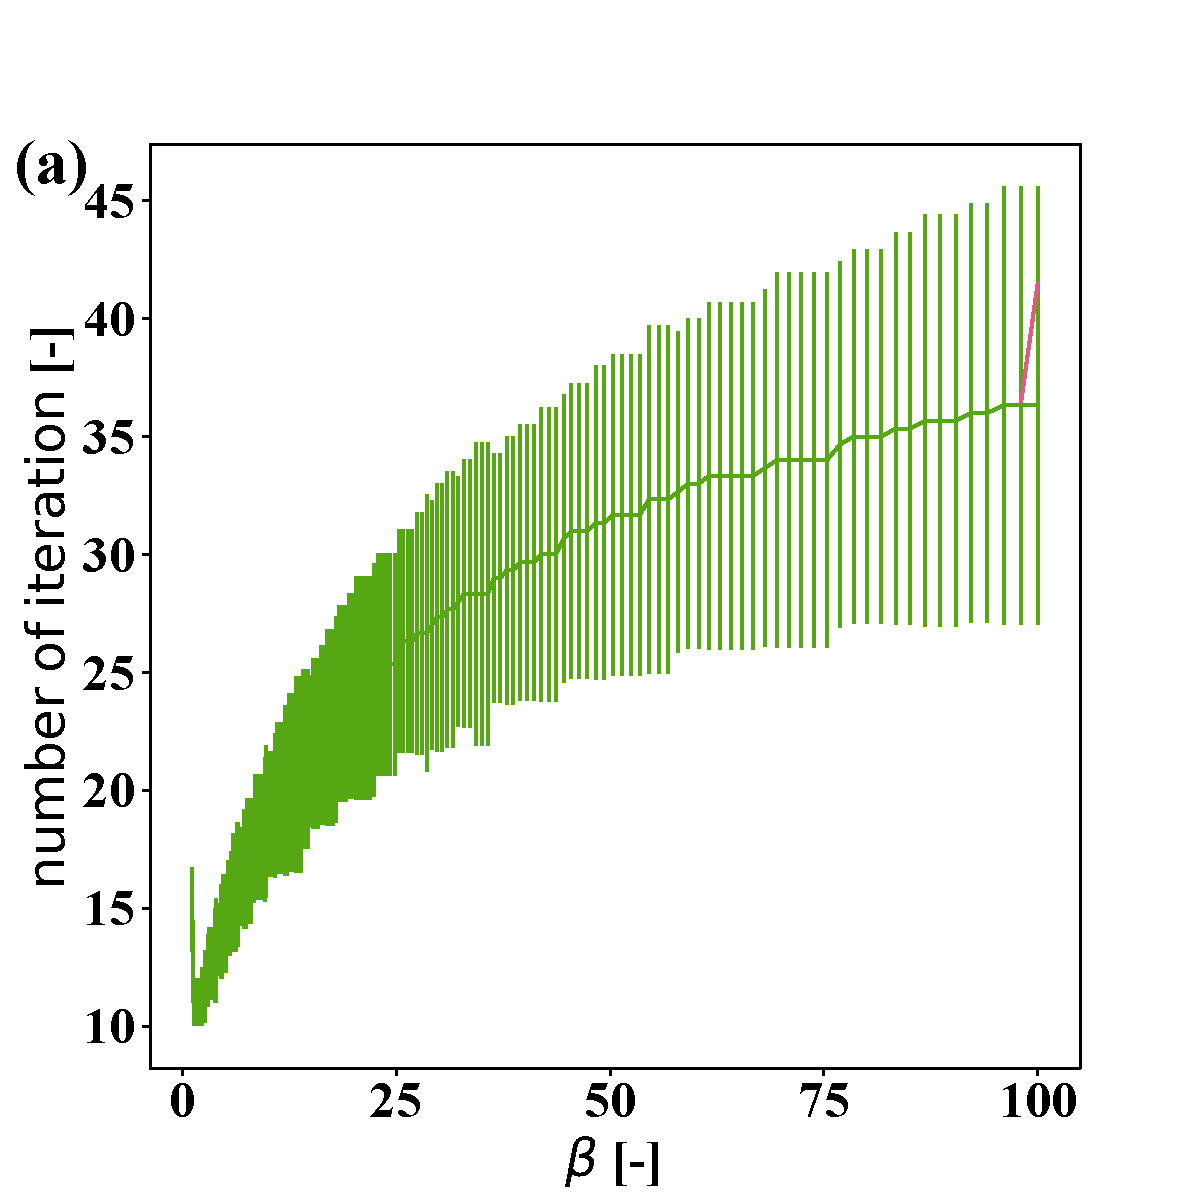
\includegraphics[width=7.0cm, height=7.0cm]{pictures/ell_homo_diff_k_sipg_it_k1.pdf}
        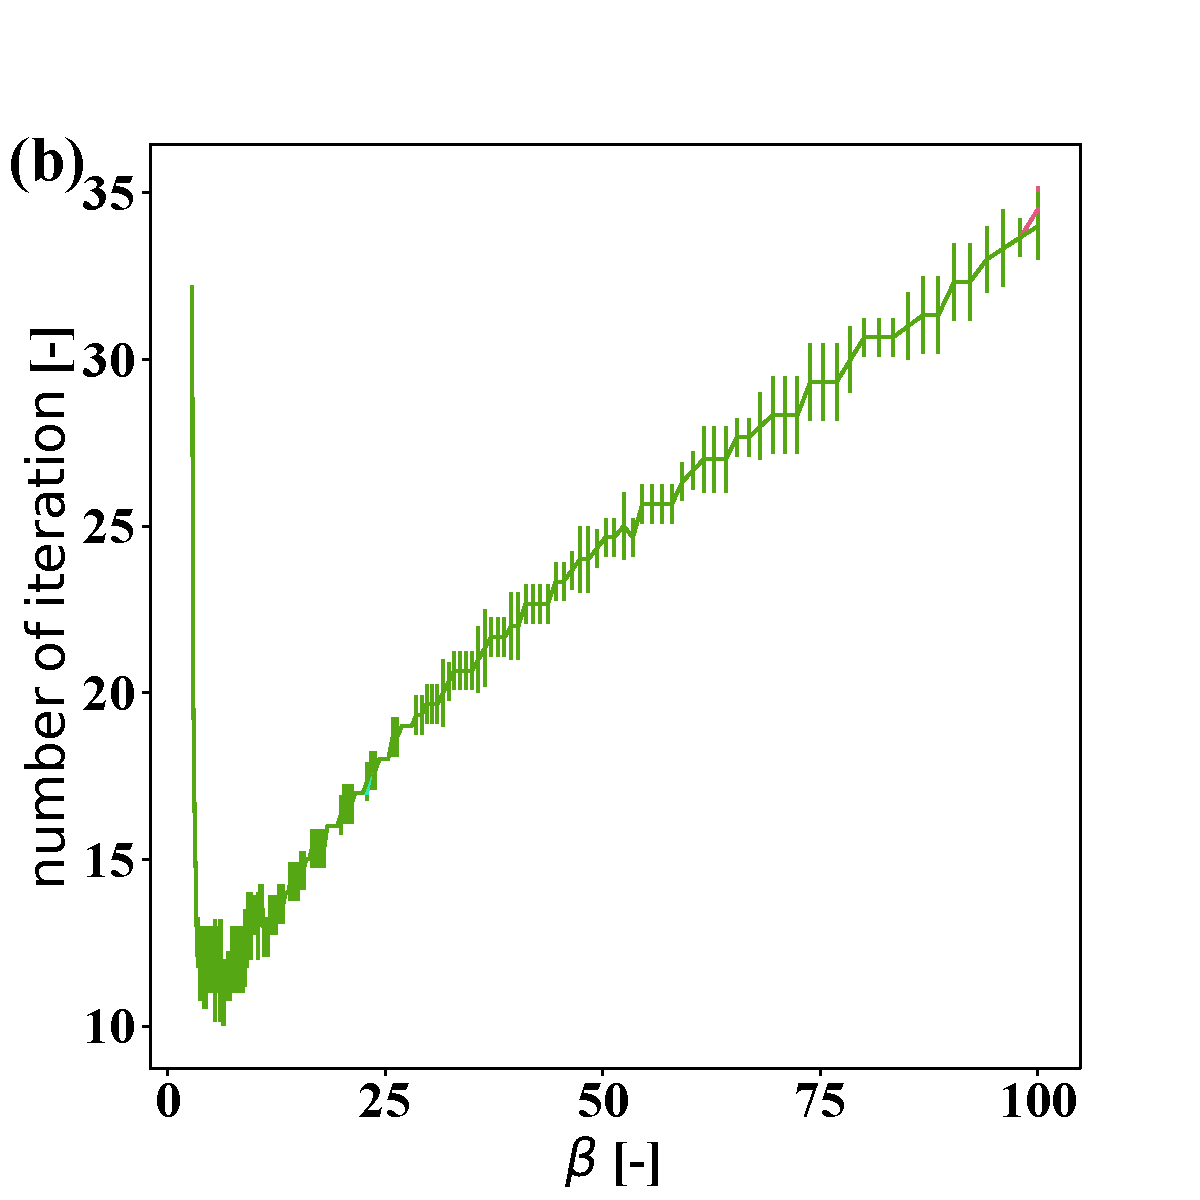
\includegraphics[width=7.0cm, height=7.0cm]{pictures/ell_homo_diff_k_sipg_it_k2.pdf}
        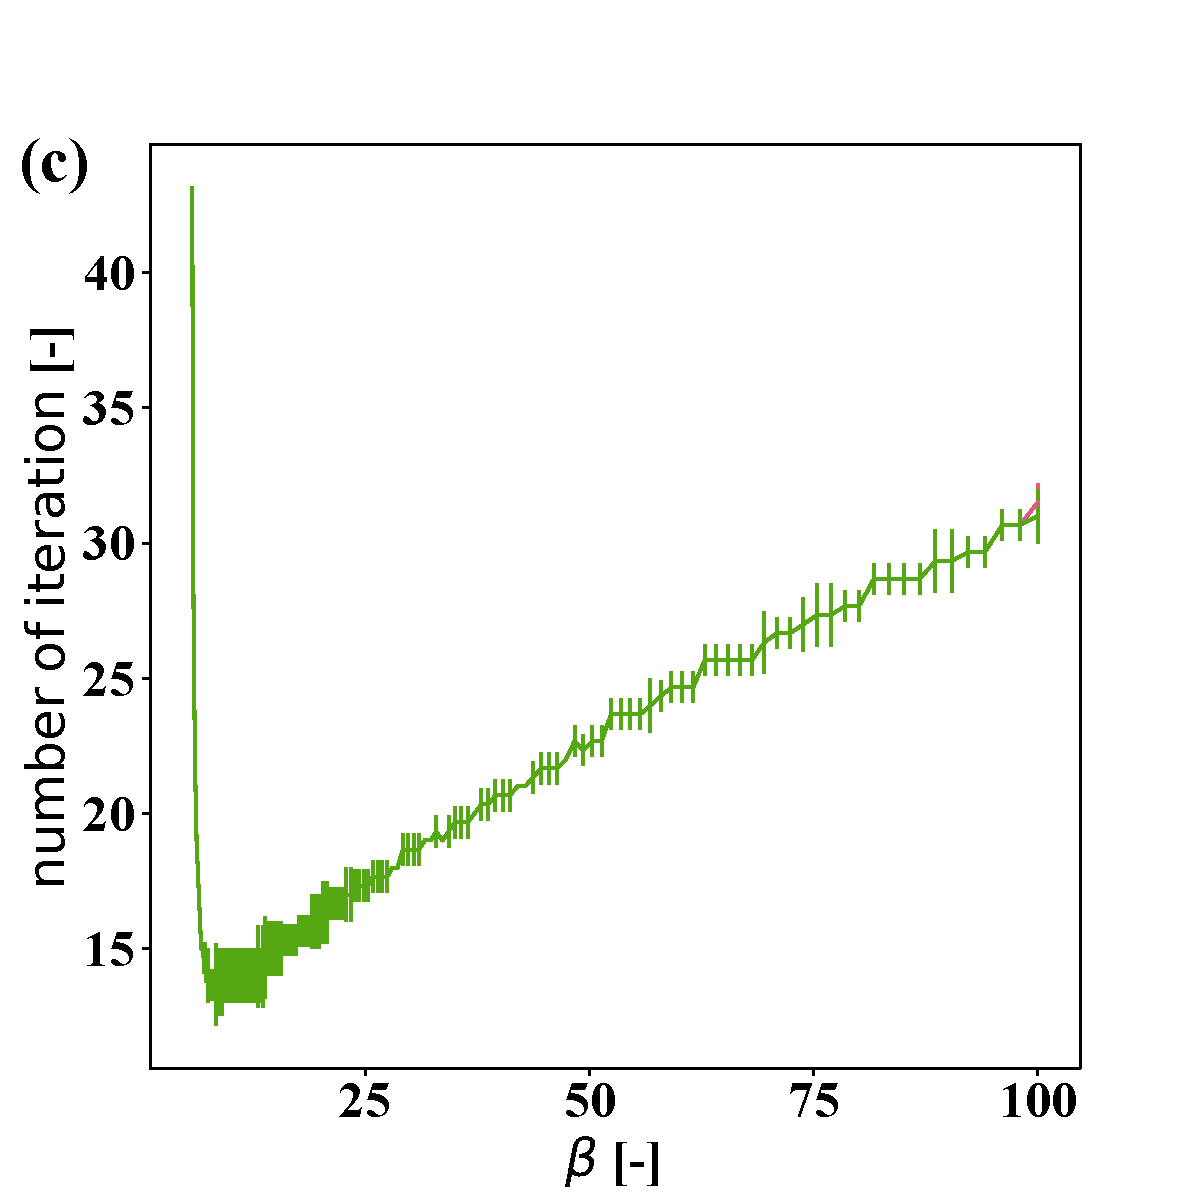
\includegraphics[width=7.0cm, height=7.0cm]{pictures/ell_homo_diff_k_sipg_it_k3.pdf}
        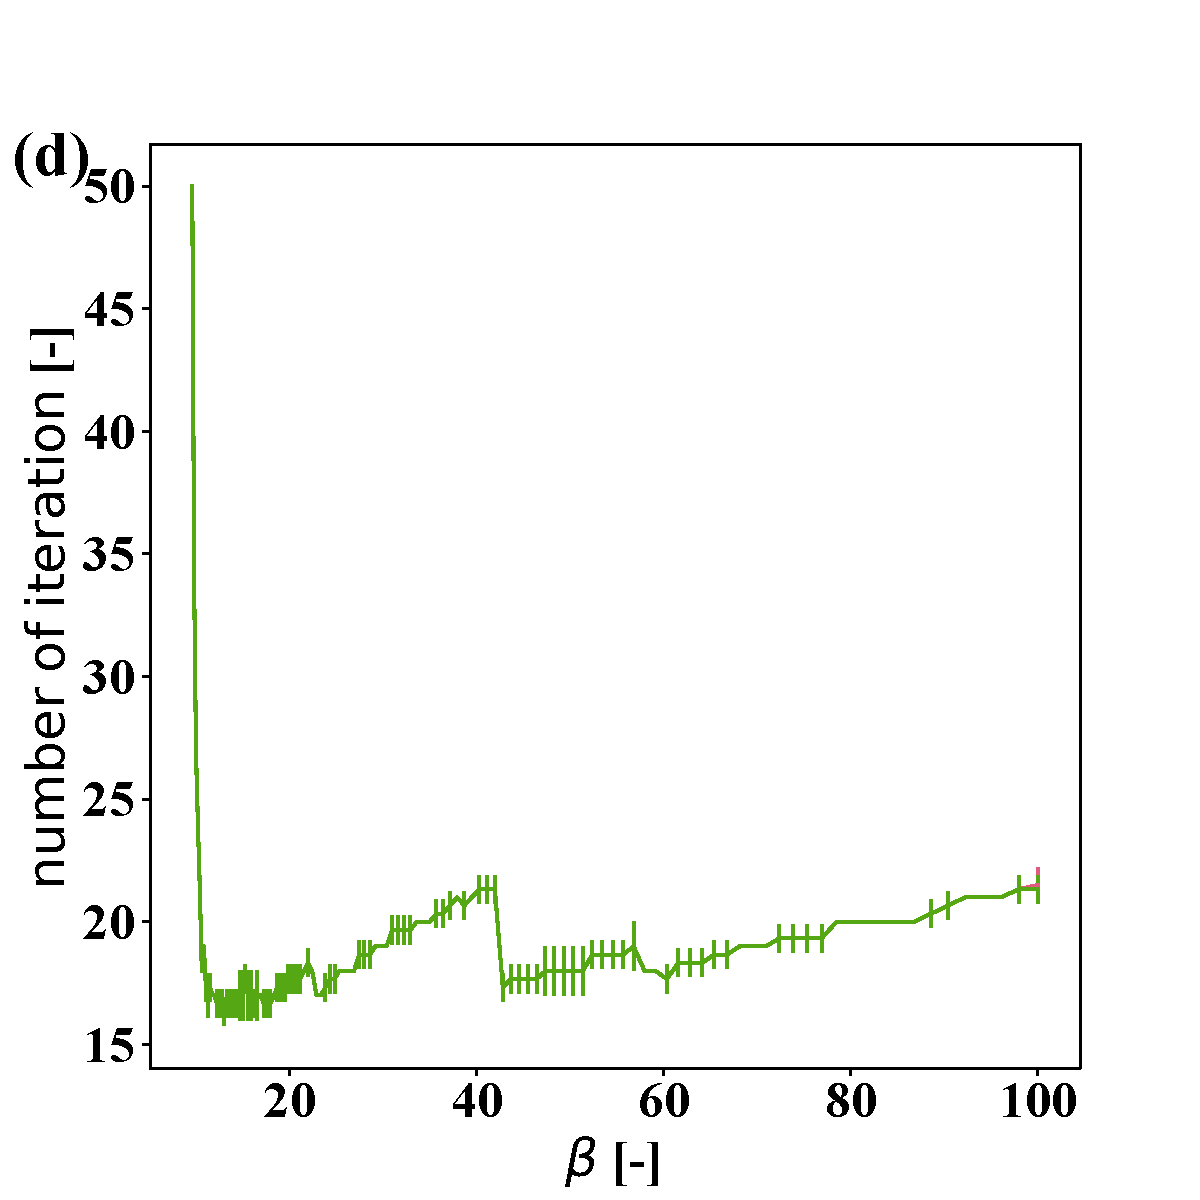
\includegraphics[width=7.0cm, height=7.0cm]{pictures/ell_homo_diff_k_sipg_it_k4.pdf}
        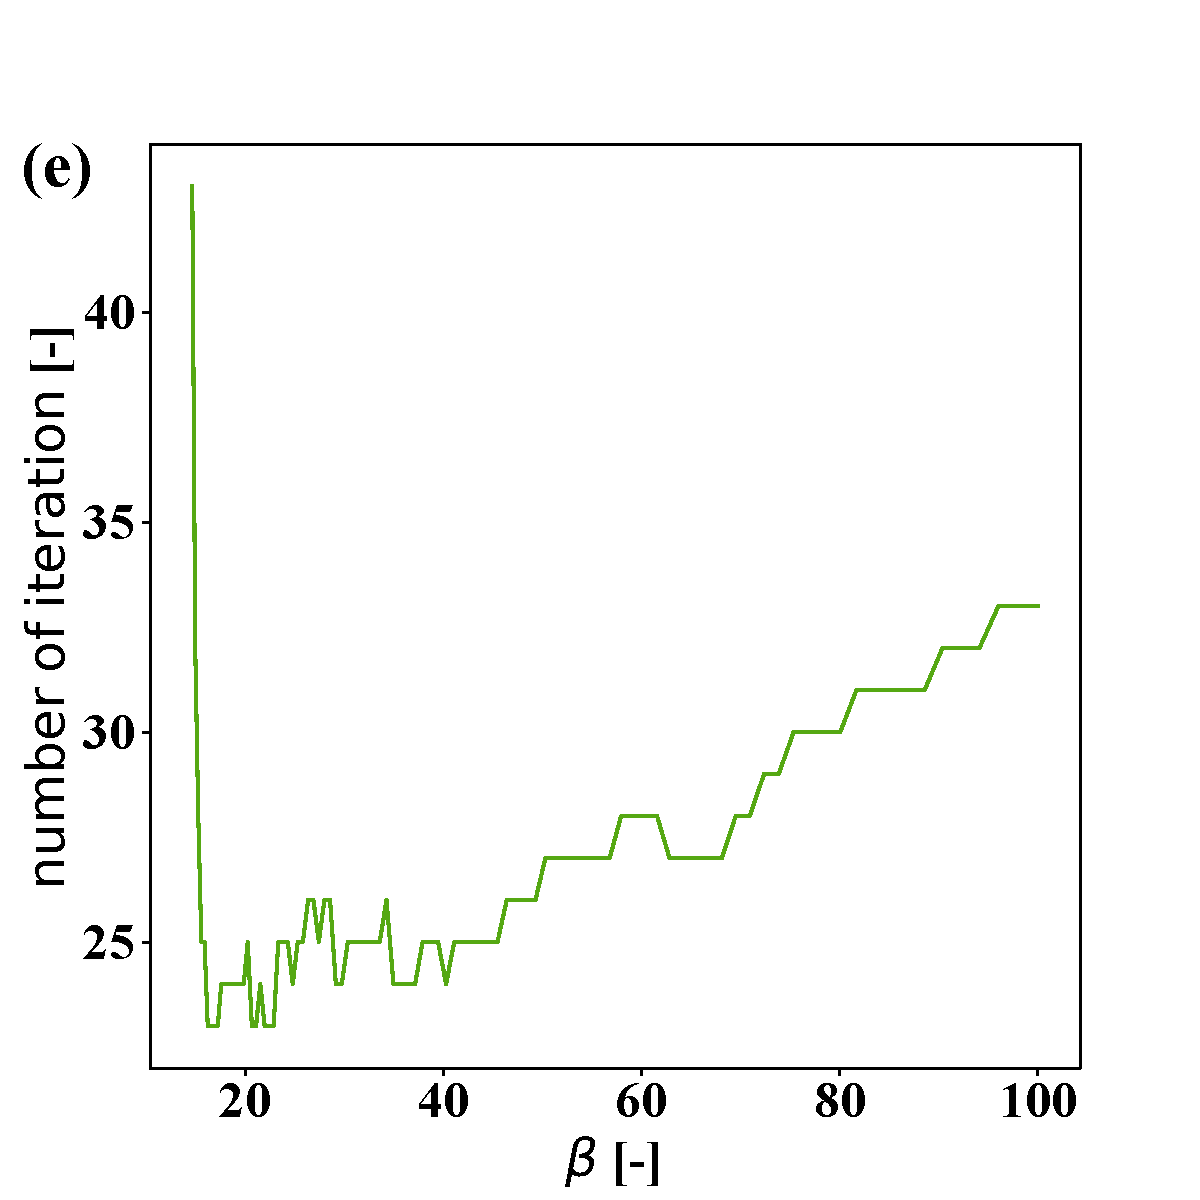
\includegraphics[width=7.0cm, height=7.0cm]{pictures/ell_homo_diff_k_sipg_it_k5.pdf}
   \caption{Number of linear iterative solver of SIPG for (\textbf{a}) $k=1$, (\textbf{b}) $k=2$, (\textbf{c}) $k=3$, (\textbf{d}) $k=4$, and (\textbf{e}) $k=5$. Note that each line represents different value of $\bm{\kappa}$, and the error bar shows mean and standard derivation of each number of iteration.}
   \label{fig:ell_homo_sipg_noi}
\end{figure}

\begin{figure}[h!]
   \centering
        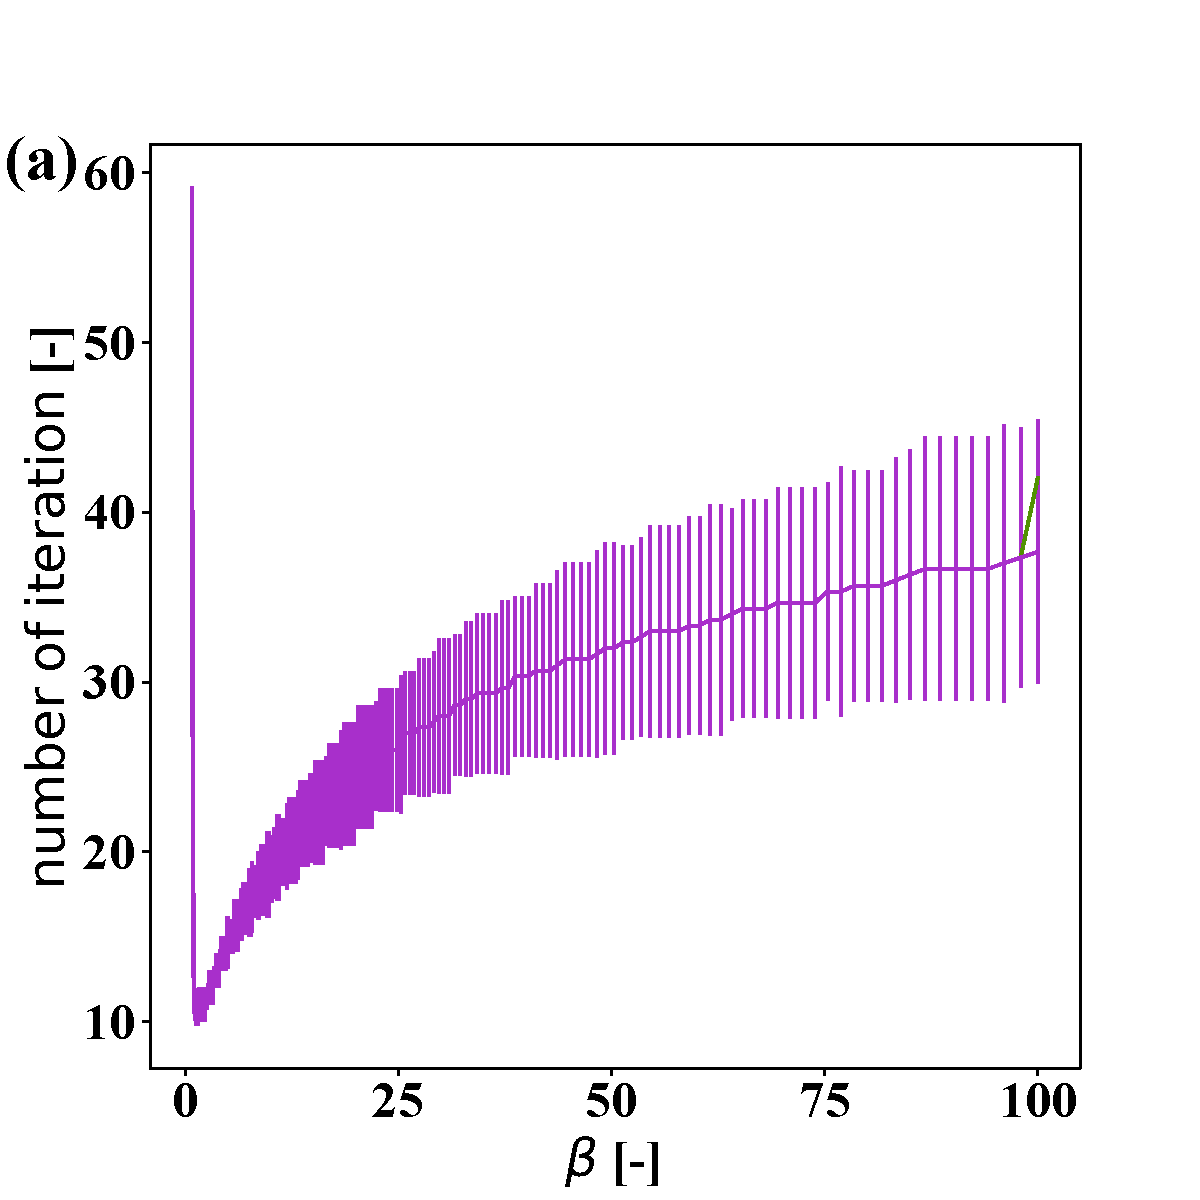
\includegraphics[width=7.0cm, height=7.0cm]{pictures/ell_homo_diff_k_iipg_it_k1.pdf}
        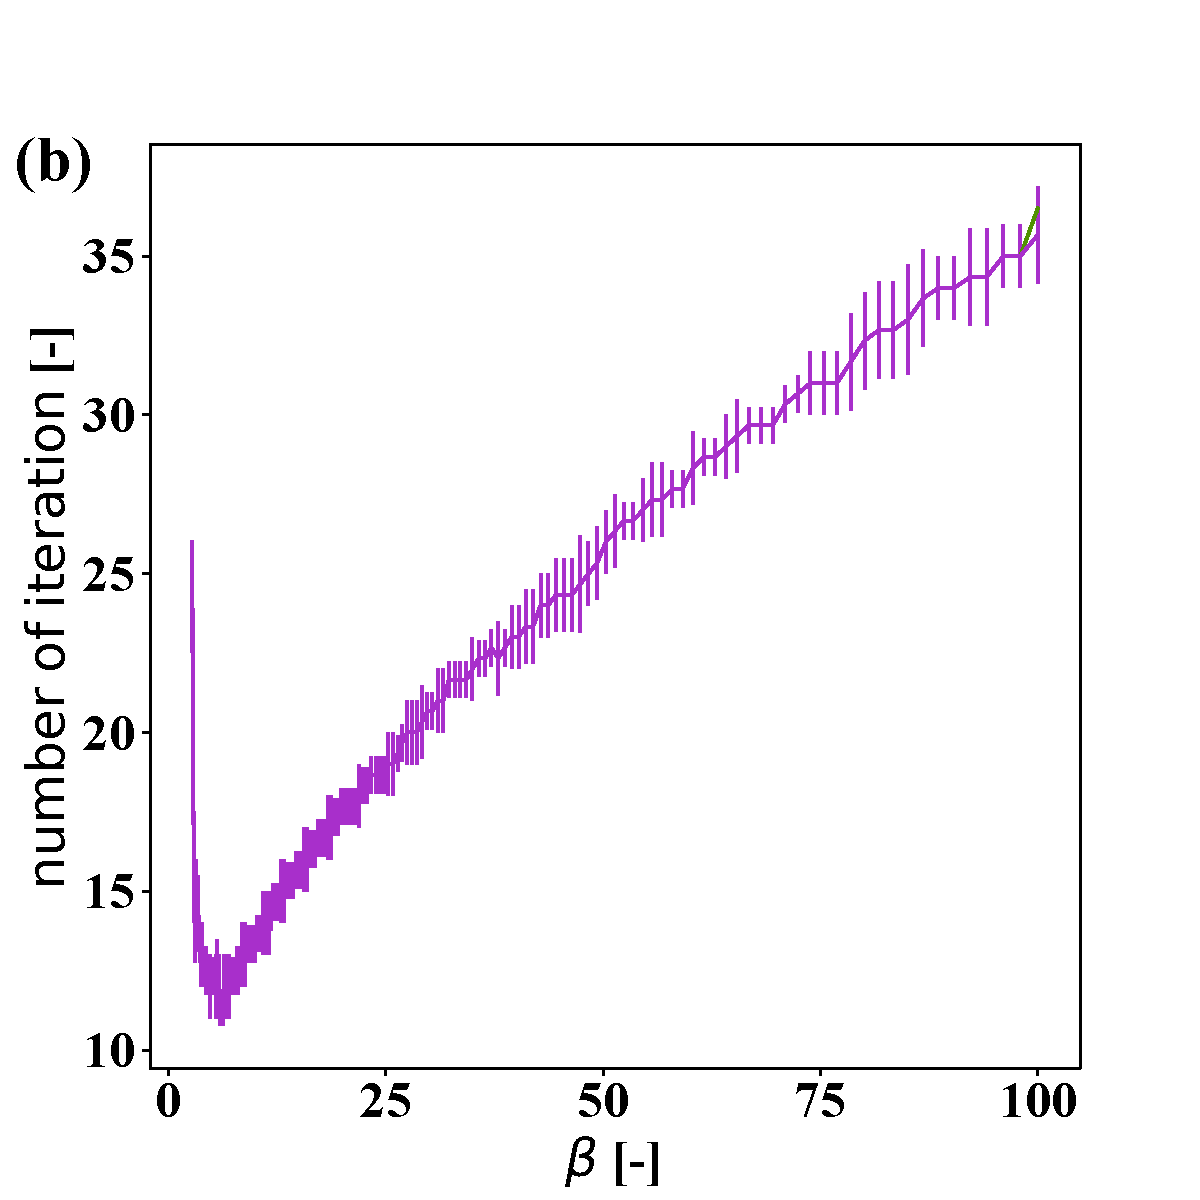
\includegraphics[width=7.0cm, height=7.0cm]{pictures/ell_homo_diff_k_iipg_it_k2.pdf}
        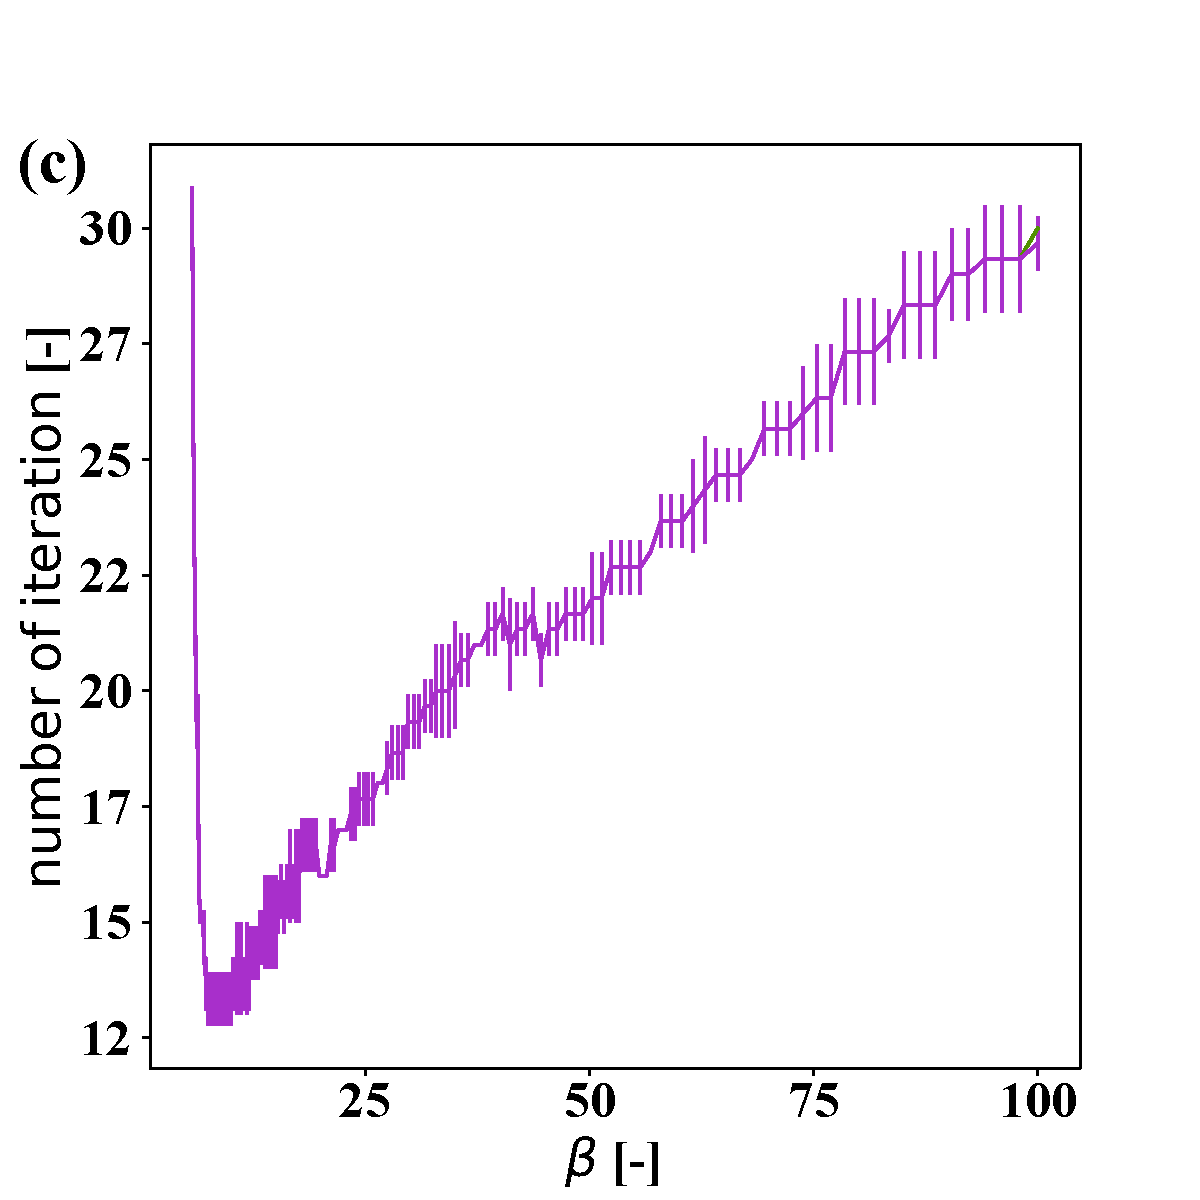
\includegraphics[width=7.0cm, height=7.0cm]{pictures/ell_homo_diff_k_iipg_it_k3.pdf}
        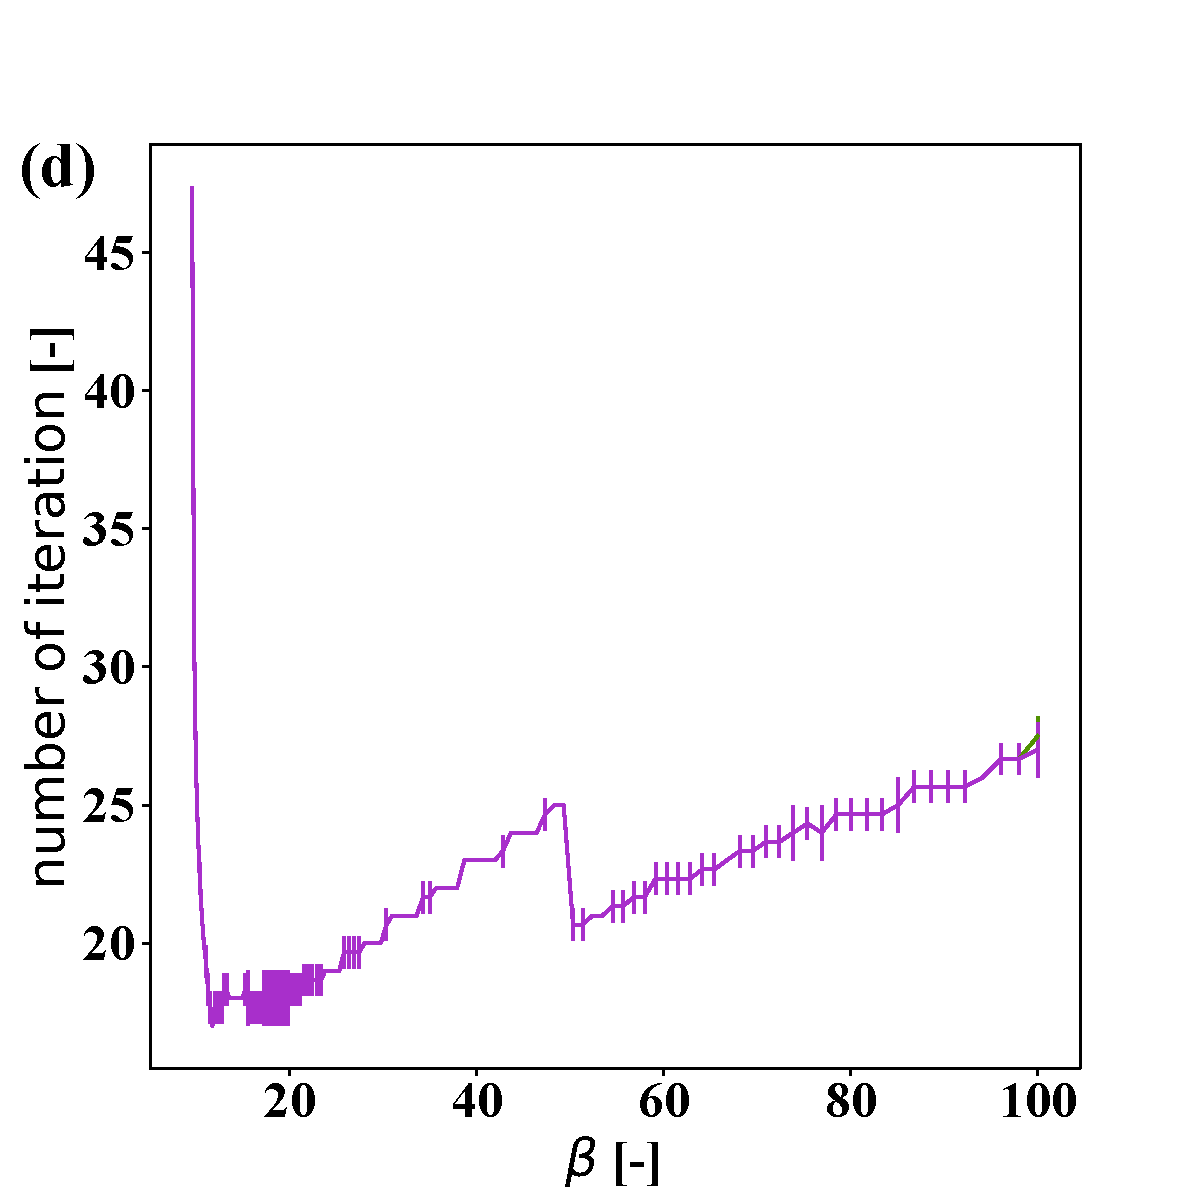
\includegraphics[width=7.0cm, height=7.0cm]{pictures/ell_homo_diff_k_iipg_it_k4.pdf}
        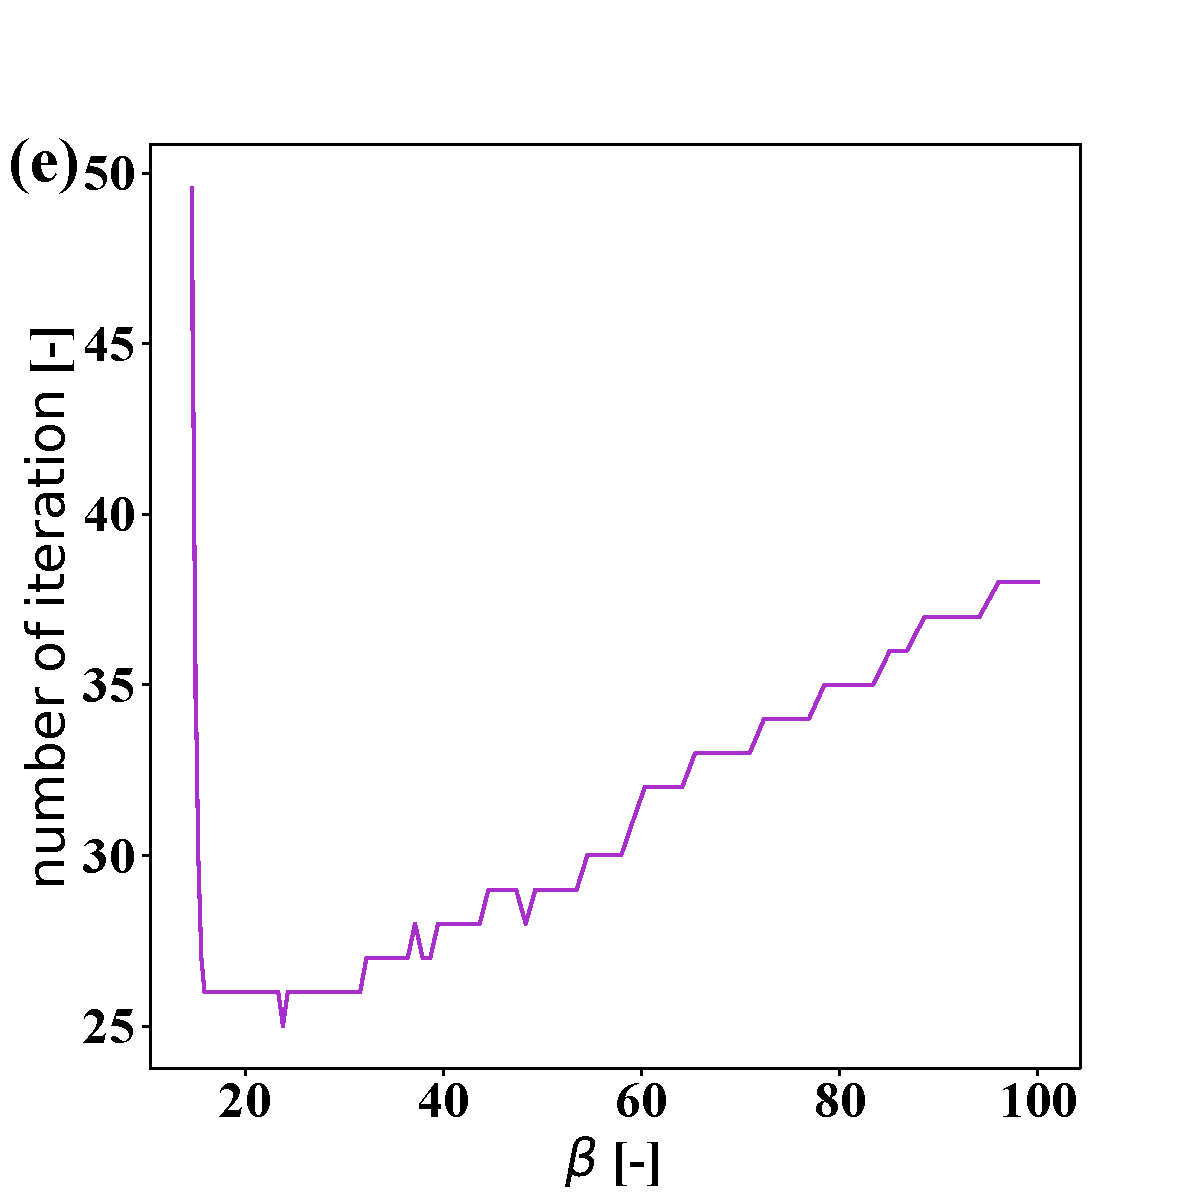
\includegraphics[width=7.0cm, height=7.0cm]{pictures/ell_homo_diff_k_iipg_it_k5.pdf}
   \caption{Number of linear iterative solver of IIPG for (\textbf{a}) $k=1$, (\textbf{b}) $k=2$, (\textbf{c}) $k=3$, (\textbf{d}) $k=4$, and (\textbf{e}) $k=5$. Note that each line represents different value of $\bm{\kappa}$, and the error bar shows mean and standard derivation of each number of iteration.}
   \label{fig:ell_homo_iipg_noi}
\end{figure}

\subsection{Biot}

\meen{As discussed, we will show only the result of SIPG with direct solver.}

\bibliography{lit}


\end{document}
